\section{Virtual Machines Preparation II}

\centeredlargetext{white}{black}{
Virtual Machine Preparation II
}

\subsection{Booting the Virtual Machine}
\begin{frame}
\frametitle{Booting the Virtual Machine}
\begin{itemize}
\item Click on the ``ITKv4'' icon on the left, to select it.
\item Click on the Green Arrow at the top ``Show''.
\item The VM will start to boot and you will see the warning:
\end{itemize}
\begin{center}
  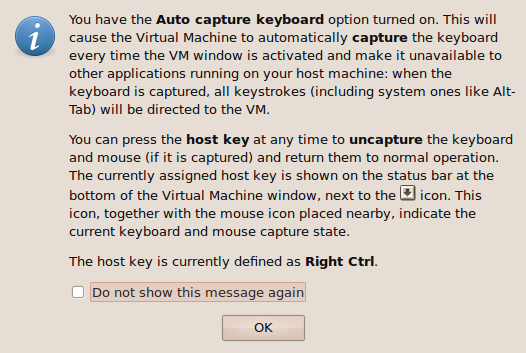
\includegraphics[width=0.4\paperwidth]{../Art/Screenshot-VirtualBox-OSE-02.png}
\end{center}
\begin{itemize}
\item Click ``OK''
\end{itemize}
\end{frame}

\begin{frame}
\frametitle{Booting the Virtual Machine}
\begin{itemize}
\item The boot sequence should continue and you should see:
\end{itemize}
\begin{center}
  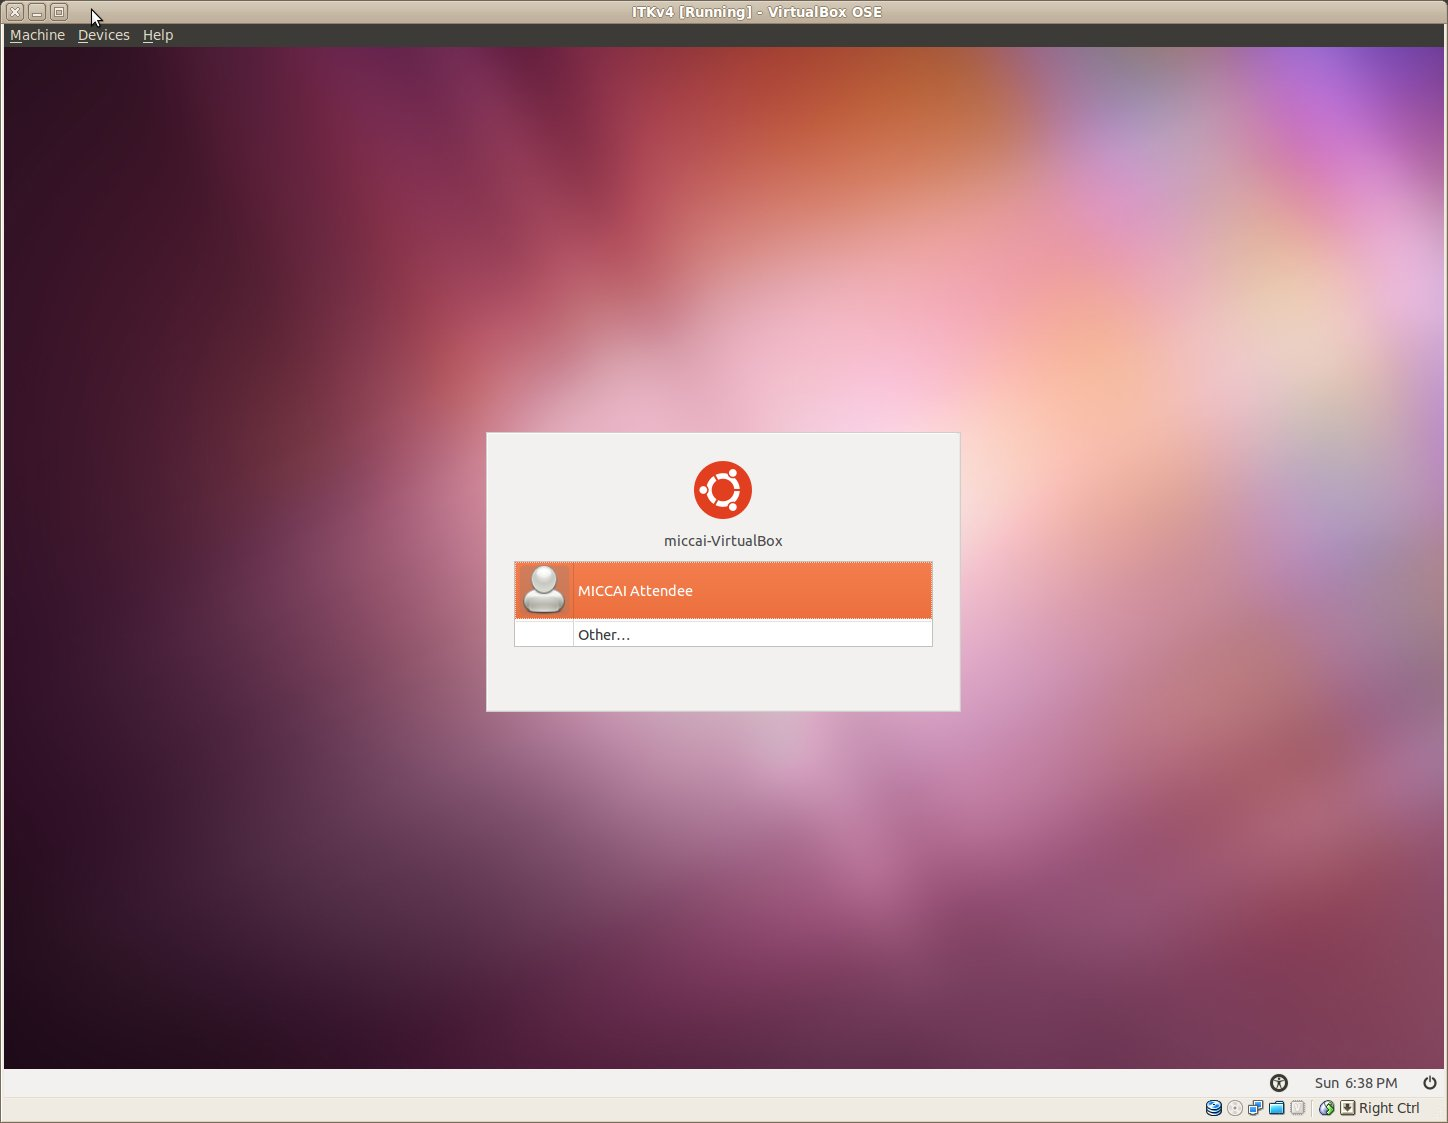
\includegraphics[width=0.7\paperwidth]{../Art/Screenshot-ITKv4-VirtualBox-01.jpg}
\end{center}
\begin{itemize}
\item Login with the password: ``toronto''
\end{itemize}
\end{frame}

\begin{frame}
\frametitle{Booting the Virtual Machine}
\begin{itemize}
\item After logging in you should see:
\end{itemize}
\begin{center}
  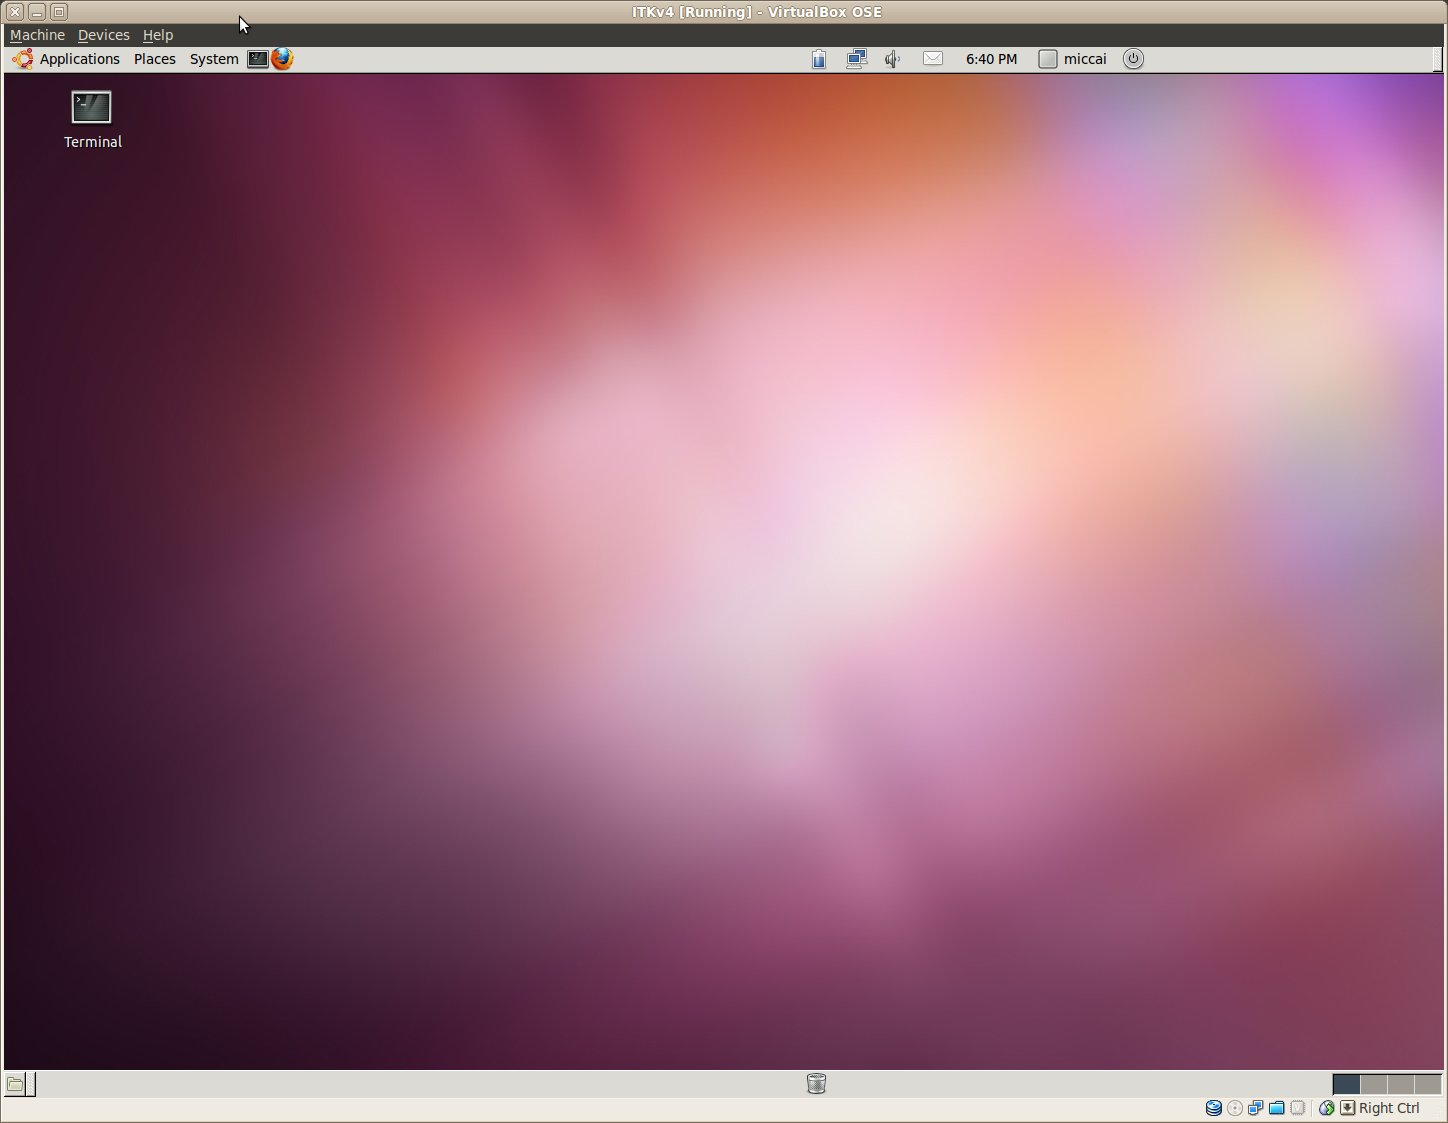
\includegraphics[width=0.7\paperwidth]{../Art/Screenshot-ITKv4-VirtualBox-02.jpg}
\end{center}
\end{frame}


\centeredlargetext{white}{black}{
Your Virtual Machine\\ is Ready !
}

\begin{frame}
\frametitle{Additional Copies}
\begin{itemize}
\item The same source trees are available in the DVD / USB key
\item Outside of the VirtualBox image
\end{itemize}
\end{frame}

\subsection{Software Environment}

\centeredlargetext{white}{black}{
Software Environment
}

{
\setbeamertemplate{background}{}
\begin{frame}
\frametitle{Welcome to Debian GNU/Linux}
\begin{center}

\includegraphics[height=0.5\paperheight]{../Art/Tux.png}
%
\includegraphics[width=0.5\paperwidth]{../Art/blackeubuntulogo.png}
\end{center}
\end{frame}
}

{
\setbeamertemplate{background}{}
\begin{frame}
\frametitle{How to take the mouse out of the Virtual Machine}
\begin{itemize}
\item Hit the \textbf{RIGHT CTRL} Key on Windows / Linux Host
\item Hit the \textbf{LEFT APPLE} Key on Mac Host
\end{itemize}
\end{frame}
}

{
\setbeamertemplate{background}{}
\begin{frame}
\frametitle{How to Open a Terminal - Menu in Lower Left Corner}
\framesubtitle{To type your command line instructions}
\begin{center}
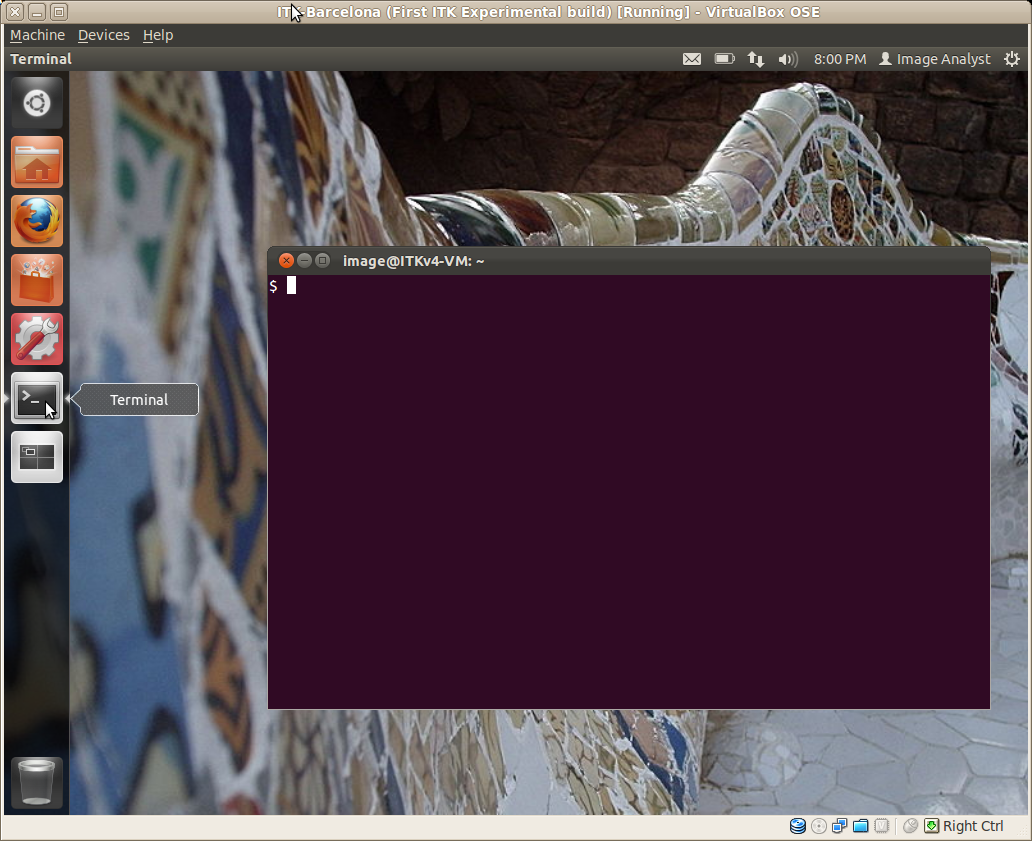
\includegraphics[width=0.7\paperwidth]{../Art/Screenshot-OpenTerminal.jpg}
\end{center}
\end{frame}
}

{
\setbeamertemplate{background}{}
\begin{frame}
\frametitle{How to Navigate Directories}
\framesubtitle{Double Click in Folder Icons in the Desktop}
\begin{center}
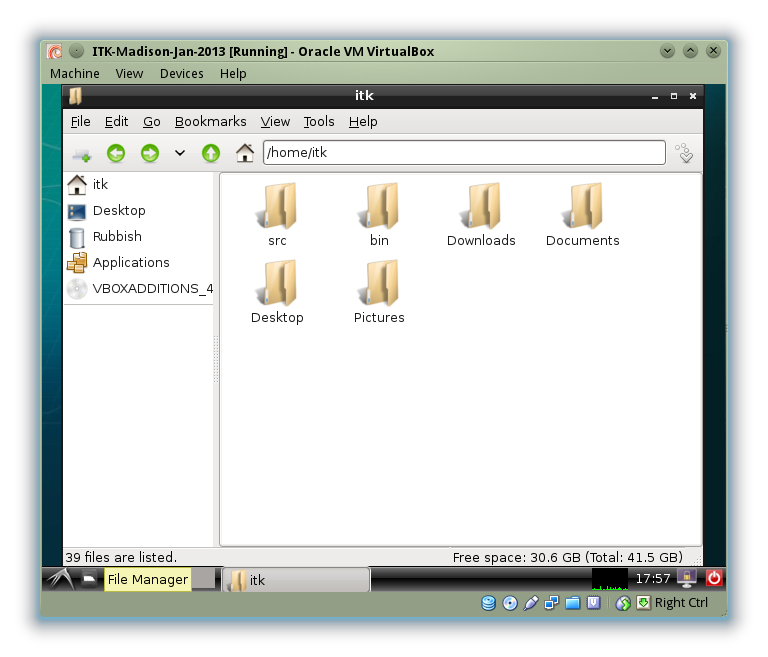
\includegraphics[width=0.7\paperwidth]{../Art/Screenshot-PCManFM.png}
\end{center}
\end{frame}
}

{
\setbeamertemplate{background}{}
\begin{frame}[fragile]
\frametitle{Walk through the directories}
\begin{itemize}
\item Find source code of exercises
\begin{verbatim}
cd ~/src/ITKv4-TheNextGeneration-Tutorial/Exercises
pwd
ls
pcmanfm .
\end{verbatim}
\pause
\item Find binary build of exercises
\begin{verbatim}
cd ~/bin/ITKv4-TheNextGeneration-Tutorial/Exercises
pwd
ls
\end{verbatim}
\end{itemize}
\end{frame}
}

{
\setbeamertemplate{background}{}
\begin{frame}[fragile]
\frametitle{The TAB Key is your Friend}
\begin{itemize}
\item When writing filenames
\item Use the TAB key for completions
\item No need to type full filenames
\end{itemize}
\end{frame}
}

{
\setbeamertemplate{background}{}
\begin{frame}[fragile]
\frametitle{How to View Images}
\begin{itemize}
\item Go to the directory
\item Invoke ``ImageViewer'' application
\begin{verbatim}
cd ~/data
ImageViewer BrainProtonDensitySlice.png
\end{verbatim}
\pause
\item Hit ``+'' key to zoom in
\pause
\item Hit ``-'' key to zoom out
\pause
\item Hit ESC key to quit the application
\end{itemize}
\end{frame}
}


